\documentclass[11pt]{article}
\usepackage[margin=1in]{geometry}
\usepackage{amsmath,amssymb,amsthm}
\usepackage{algorithm}
\usepackage{algpseudocode}
\usepackage{graphicx}
\usepackage{booktabs}
\usepackage{listings}
\usepackage{xcolor}
\usepackage{url}
\usepackage[hidelinks]{hyperref}

\graphicspath{{../figures/}}
% \input inside tabular breaks \bottomrule; use the primitive instead.
\makeatletter\newcommand{\tabinput}[1]{\@@input #1 }\makeatother
\newtheorem{lemma}{Lemma}
\newtheorem{theorem}{Theorem}

\lstset{basicstyle=\ttfamily\scriptsize, breaklines=true, columns=fullflexible,
        keywordstyle=\color{blue!60!black}\bfseries, commentstyle=\color{gray},
        numbers=left, numberstyle=\tiny\color{gray}, frame=single, language=Java,
        literate={·}{{$\cdot$}}1 {×}{{$\times$}}1 {δ}{{$\delta$}}1}

\newcommand{\SOneLen}{25.9}
\newcommand{\SOneMis}{0.4}
\newcommand{\SOneScore}{21.5}


\title{Analysis of Algorithms: Assignment 2\\Dynamic Programming}
\author{Surya Charan Perisetla}
\date{}

\begin{document}
\maketitle

\section*{Overview}
This report designs, analyses, implements and evaluates two dynamic-programming
(DP) algorithms: a weighted approximate common substring without gaps
(Problem~1) and the largest all-zero square sub-matrix of a boolean matrix
(Problem~2). Both are implemented in Java with iterative loops and arrays only
(no recursion), including the extraction of the optimal solution. Every
number in this report is produced by \texttt{run\_experiments.py}, which
builds the programs, runs the tests and experiments and redraws all figures and
tables. Experiments ran on an Apple-silicon Mac with OpenJDK~25
(\texttt{java -Xmx2g}). Every timed method is warmed up first so that the
JIT compiler has finished before it is measured.

\paragraph{Notation and scenarios.} We write $w_c$ for the weight of letter
$c$ and $\delta \ge 0$ for the size of the mismatch penalty (each mismatch
adds $-\delta$ to the score). The assignment defines two scenarios.
\emph{Scenario~1}: every letter has weight $w_c=1$, and $\delta=10$.
\emph{Scenario~2}: $w_c$ is proportional to the
frequency of $c$ in English, and $\delta$ takes 10 values between
$\min_c w_c$ and $\max_c w_c$. As an additional experiment
(Section~\ref{sec:s1sweep}) we also run Scenario~1 with other penalties,
$\delta\in\{1,2,3,4,5,6,8,10\}$, to show how the penalty changes the result.

%======================================================================
\section{Problem 1: Weighted Approximate Common Substring}
%======================================================================

\subsection{Problem statement}
Let $X = x_1 \dots x_n$ and $Y = y_1 \dots y_m$ be strings over
$\Sigma = \{A,\dots,Z\}$. Define the per-position score
\[
  s(a,b) = \begin{cases} w_a & a = b,\\ -\delta & a \ne b. \end{cases}
\]
A candidate solution is a triple $(i,j,L)$ with $L\ge 1$, $i+L-1\le n$ and
$j+L-1\le m$, describing the equal-length (gap-free) substrings
$X[i..i+L-1]$ and $Y[j..j+L-1]$. Its score is
\[
  \mathrm{score}(i,j,L) \;=\; \sum_{t=0}^{L-1} s(x_{i+t},\, y_{j+t}),
\]
that is, the sum of the weights of the matching letters minus $\delta$ for each
mismatch. We want $\max_{(i,j,L)} \mathrm{score}(i,j,L)$ and a triple that
attains it. In the assignment example, $X=$\texttt{ABCAABCAA},
$Y=$\texttt{ABBCAACCBBBBBB}, the pair \texttt{CAABC}/\texttt{CAACC} at
$(3,4,5)$ scores $2w_C+2w_A-\delta$. Our test suite checks this value.

\subsection{Optimisation function and Bellman equations}
Indexing by the \emph{end} of the alignment gives the subproblems:
\[
  \mathrm{OPT}(i,j) \;=\; \max_{1\le L\le \min(i,j)} \; \sum_{t=0}^{L-1} s(x_{i-t},\, y_{j-t}),
  \qquad 1\le i\le n,\; 1\le j\le m,
\]
which is the best score of a gap-free pair of substrings ending exactly at
$x_i$ and $y_j$. The recurrence (the Bellman equations) is
\begin{align*}
  \mathrm{OPT}(i,j) &= s(x_i,y_j) + \max\bigl(0,\; \mathrm{OPT}(i-1,j-1)\bigr), \qquad i,j\ge 1,\\
  \mathrm{OPT}(0,j) &= \mathrm{OPT}(i,0) = 0 \quad\text{(boundary, ``no predecessor'')},
\end{align*}
and the answer is
\[
  \mathrm{OPT}^\ast = \max_{1\le i\le n,\;1\le j\le m} \mathrm{OPT}(i,j).
\]
Along each diagonal $i-j=\text{const}$ this is exactly Kadane's maximum-subarray
recurrence applied to the sequence $s(x_1,y_{1+d}), s(x_2,y_{2+d}),\dots$.

\subsection{Correctness}
\begin{lemma}[Optimal substructure]
For $i,j\ge1$, $\mathrm{OPT}(i,j) = s(x_i,y_j) + \max(0, \mathrm{OPT}(i-1,j-1))$,
with $\mathrm{OPT}(i-1,j-1)$ read as $0$ when $i=1$ or $j=1$.
\end{lemma}
\begin{proof}
Every candidate ending at $(i,j)$ has length $L=1$ or $L\ge2$.
If $L=1$ its score is $s(x_i,y_j)$.
If $L\ge2$ (possible only when $i,j\ge2$) its score is
$s(x_i,y_j)$ plus the score of a candidate of length $L-1$ ending at
$(i-1,j-1)$. Conversely, every candidate ending at $(i-1,j-1)$ extends by one
position to a candidate ending at $(i,j)$. Therefore the best candidate of
length $\ge2$ scores exactly $s(x_i,y_j)+\mathrm{OPT}(i-1,j-1)$, and
\[
\mathrm{OPT}(i,j) = \max\bigl(s(x_i,y_j),\; s(x_i,y_j)+\mathrm{OPT}(i-1,j-1)\bigr)
               = s(x_i,y_j)+\max(0,\mathrm{OPT}(i-1,j-1)).
\]
On the boundary ($i=1$ or $j=1$) only $L=1$ is possible, and reading the
boundary value as $0$ gives $s(x_i,y_j)$.
\end{proof}
\begin{theorem}
The algorithm returns $\mathrm{OPT}^\ast$ and a triple attaining it.
\end{theorem}
\begin{proof}
Cells are filled in row-major order, so $(i-1,j-1)$ is always computed before
$(i,j)$. By induction on $i+j$ and the lemma, every table entry
$S[i][j]$ equals $\mathrm{OPT}(i,j)$. Every candidate ends at some
$(i,j)$, so the maximum over all entries is $\mathrm{OPT}^\ast$. Extraction
(below) follows the choices that produced that entry and so recovers a
candidate with exactly that score.
\end{proof}

\subsection{Extracting the optimal substring}
During the fill we record the end cell $(i^\ast,j^\ast)$ of the maximum
(the first one in row-major order if there are ties). In the lemma, the
predecessor $(i-1,j-1)$ was used exactly when $\mathrm{OPT}(i-1,j-1)>0$. So
we walk up the diagonal:
\begin{algorithmic}[1]
\State $i\gets i^\ast$, $j\gets j^\ast$
\While{$i>1$ \textbf{and} $j>1$ \textbf{and} $S[i-1][j-1] > 0$}
  \State $i\gets i-1$; $j\gets j-1$
\EndWhile
\State \Return start $(i,j)$, length $L=i^\ast-i+1$
\end{algorithmic}
The reported substrings are $X[i..i^\ast]$ and $Y[j..j^\ast]$. The number of
mismatches is counted by comparing them. An optimal solution never starts or
ends with a mismatch unless it has length~1, because removing that position
would raise the score.

We also implemented a \emph{linear-space} variant. It keeps two rolling rows of
$S$ plus, for each cell, the run length $\ell[i][j]$ ($=\ell[i-1][j-1]+1$ if the
predecessor is used, else $1$). It reports the same answer as the full table,
with the same tie-breaking, without storing the table: start $=(i^\ast-\ell+1,\,j^\ast-\ell+1)$.

\begin{algorithm}[h]
\caption{Weighted approximate common substring (full table)}
\begin{algorithmic}[1]
\State allocate $S[0..n][0..m]$, all $0$; $\mathit{best}\gets-\infty$
\For{$i \gets 1$ \textbf{to} $n$}
  \For{$j \gets 1$ \textbf{to} $m$}
    \State $S[i][j] \gets s(x_i,y_j) + \max(0, S[i-1][j-1])$
    \If{$S[i][j] > \mathit{best}$} $\mathit{best}\gets S[i][j]$; $(i^\ast,j^\ast)\gets(i,j)$ \EndIf
  \EndFor
\EndFor
\State traceback from $(i^\ast,j^\ast)$ as above
\end{algorithmic}
\end{algorithm}

\subsection{Time and space complexity}
\begin{itemize}
\item \textbf{Time} $\Theta(nm)$. There are $nm$ cells, each computed in $O(1)$
  (one comparison, one lookup of $w$, one addition, one max). Traceback walks
  at most $\min(n,m)$ diagonal steps, and counting mismatches takes $O(L)$. Both
  are dominated by $nm$.
\item \textbf{Space} $\Theta(nm)$ for the full table: $(n+1)(m+1)$ doubles,
  that is $8(n+1)(m+1)$ bytes, plus $O(n+m)$ for the input. The linear variant needs
  $\Theta(m)$: two rows of doubles and two rows of ints, $24(m+1)$ bytes.
  Swapping $X$ and $Y$ makes this $\Theta(\min(n,m))$.
\end{itemize}

\subsection{Synthetic data and experiments}
\paragraph{Weights.} Scenario~1: $w_c=1$, $\delta=10$. Scenario~2:
$w_c$ equals the relative frequency (in percent) of letter $c$ in English text,
as given by Lewand~\cite{lewand} (E $=12.702$, T $=9.056$, A $=8.167$, \dots,
Z $=0.074$). Any proportionality constant gives the same optimal substring as
long as $\delta$ is scaled by the same constant, so percentages are used. The
penalty takes the 10 evenly spaced values strictly between
$w_{\min}=0.074$ and $w_{\max}=12.702$,
$\delta_k=w_{\min}+k(w_{\max}-w_{\min})/11$ for $k=1..10$. We also report the
two endpoints.

\paragraph{Strings.} Scenario~1 strings are uniform over $\{A..Z\}$.
Scenario~2 strings are drawn letter by letter from the English frequency
distribution, so frequent letters (with large weights) also appear often. For
the $\delta$ sweep we use two data sets of $n=m=2000$, each with 10 random seeds:
\emph{random} (independent strings) and \emph{planted}. In the planted set, a
random 200-letter block of $X$ is copied into a random position of $Y$, and
each copied letter is replaced by a different random letter with probability
$0.15$. This gives a known true approximate match with about 30 mismatches.

\paragraph{Correctness tests.} \texttt{java Substring test} checks the assignment
example, edge cases (no common letter, identical strings) and 3000 random
small instances (lengths $\le30$, alphabets of 2--6 letters, both scenarios,
random $\delta$). It compares the full-table DP, the linear DP and a brute
force that enumerates every $(i,j,L)$ in $O(nm\min(n,m))$ time. It also re-scores
the extracted substring. All tests pass; the output is saved in the \texttt{results} folder.

\subsubsection{Running time and memory}
Table~\ref{tab:p1rt} and Figures~\ref{fig:p1rt}--\ref{fig:p1mem} show the
best of 3--5 runs per configuration. The time per cell is roughly constant
for large inputs: about 1.3~ns per cell in Scenario~1 and 2.1~ns in
Scenario~2. The three shapes with the same $nm=4\cdot10^6$ ($2000^2$,
$1000\times4000$, $500\times8000$) take the same time. Both observations
confirm $\Theta(nm)$ and show that only the product $nm$ matters. Full-table
memory grows as $8nm$ bytes (122~MiB at $4000\times4000$), while the linear
variant stays at a few KiB. For the smaller inputs the full table is slower
per cell than the linear variant, probably because Java must allocate and
zero the whole $8nm$-byte array (and the garbage collector must reclaim it)
before the DP starts, which the two-row version avoids.
For large inputs the two variants take the same time. Scenario~2 is slower
than Scenario~1 because the branch ``$S[i-1][j-1]>0$'' is harder for the CPU
to predict when many letters give small positive scores.

\begin{table}[h]\centering\small
\caption{Problem 1: time (ms) and DP memory as a function of input size.}\label{tab:p1rt}
\begin{tabular}{lrrrrrr}\toprule
 & \multicolumn{2}{c}{Scenario 1 (ms)} & \multicolumn{2}{c}{Scenario 2 (ms)} & \multicolumn{2}{c}{DP memory}\\
\cmidrule(lr){2-3}\cmidrule(lr){4-5}\cmidrule(lr){6-7}
$n\times m$ & full & linear & full & linear & full (MiB) & linear (KiB)\\\midrule
\tabinput{../results/p1_runtime_table.tex}
\bottomrule\end{tabular}
\end{table}

\begin{figure}[h]\centering
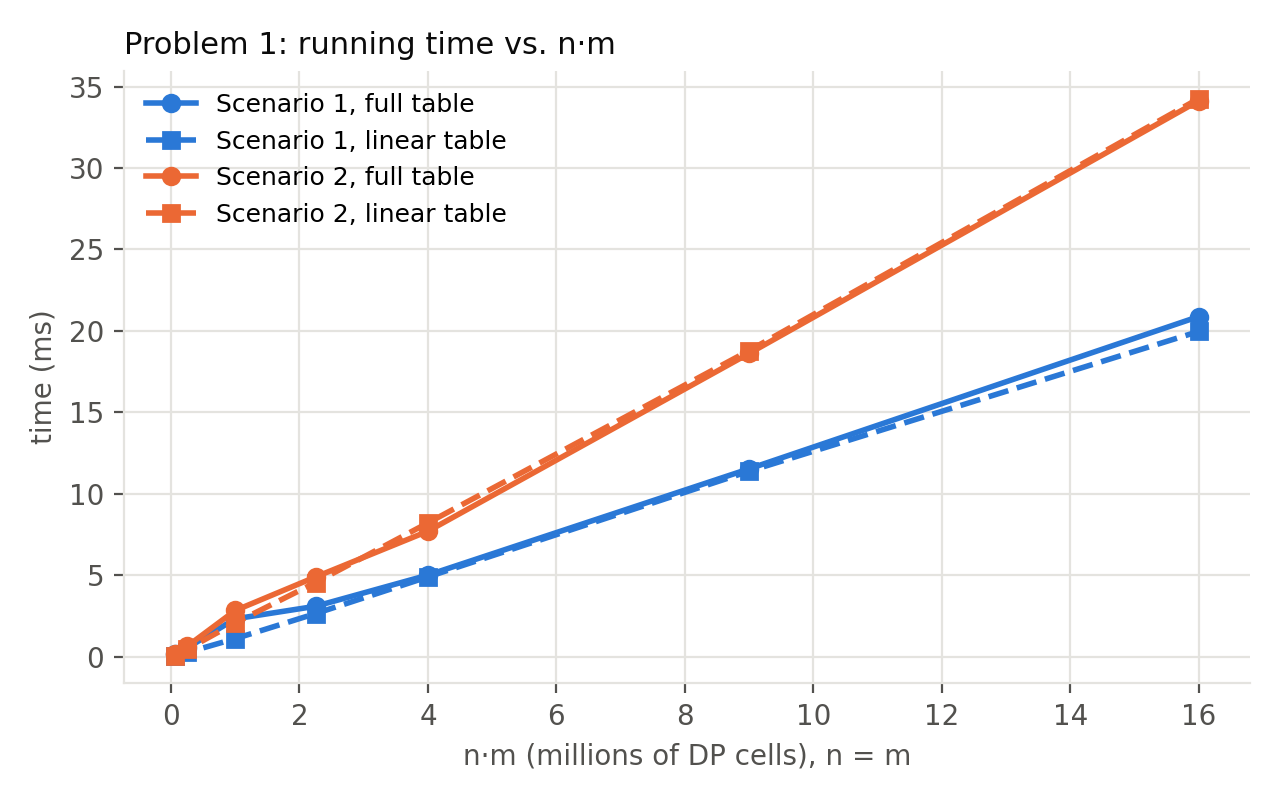
\includegraphics[width=0.49\textwidth]{p1_runtime.png}\hfill
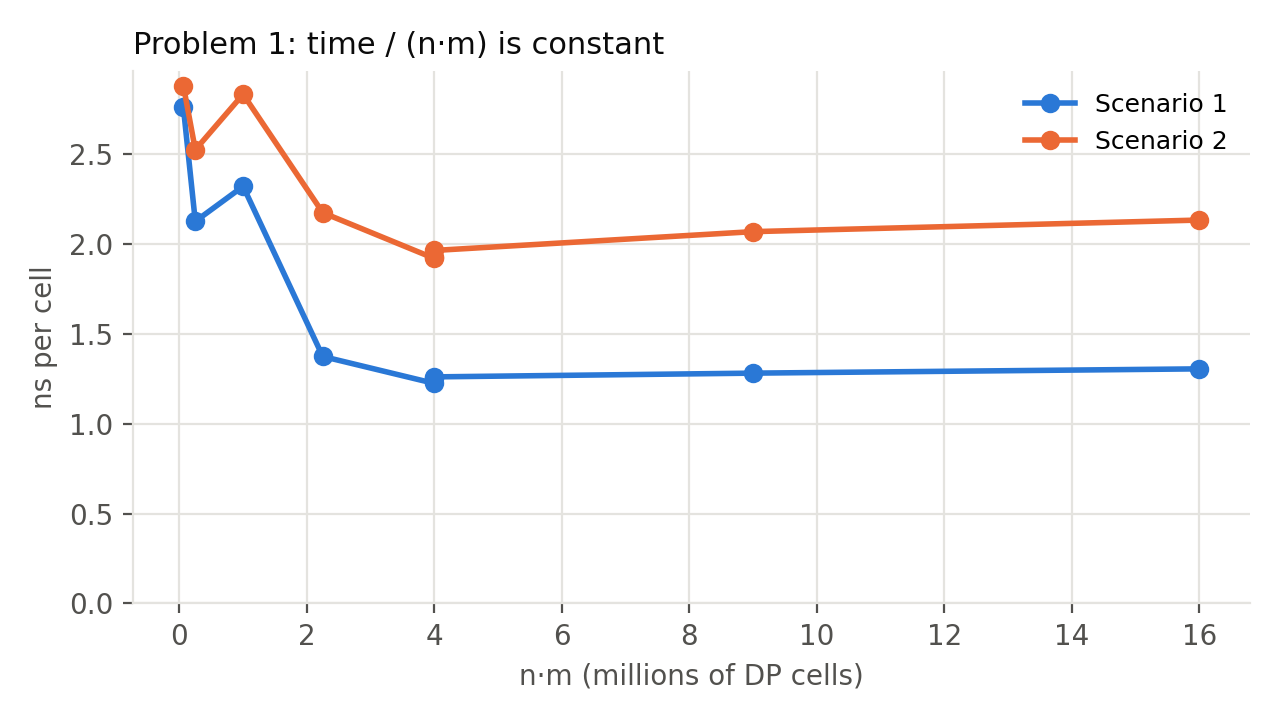
\includegraphics[width=0.49\textwidth]{p1_time_per_cell.png}
\caption{Problem 1 running time. Left: time grows linearly in $nm$. Right:
time per DP cell is flat for every input shape, including $n\ne m$.}\label{fig:p1rt}
\end{figure}

\begin{figure}[h]\centering
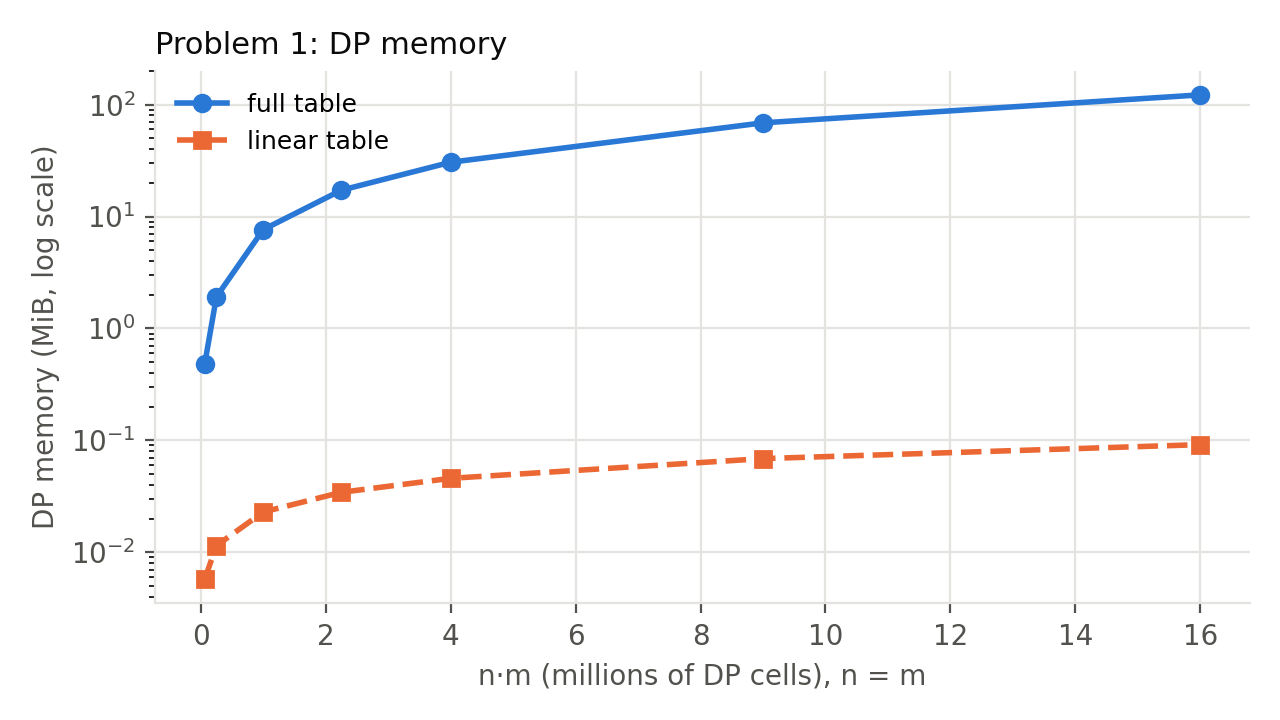
\includegraphics[width=0.6\textwidth]{p1_memory.png}
\caption{Problem 1 DP memory (log scale): $\Theta(nm)$ for the full table vs.\ $\Theta(m)$ for two rolling rows.}\label{fig:p1mem}
\end{figure}

\subsubsection{Scenario 2: effect of the mismatch penalty}
Table~\ref{tab:p1sweep} and Figure~\ref{fig:p1sweep} report means over the
10 seeds. ``Overlap'' is the number of letters of the reported substring that
lie on the planted block, on the correct diagonal.

\begin{table}[h]\centering\small
\caption{Scenario 2, $n=m=2000$, means of 10 seeds. Rows 1 and 12 are the endpoints $w_{\min}$, $w_{\max}$; rows 2--11 are the 10 required intermediate values.}\label{tab:p1sweep}
\begin{tabular}{rrrrrrrr}\toprule
 & \multicolumn{3}{c}{random strings} & \multicolumn{4}{c}{planted 200-letter block, 15\% mutated}\\
\cmidrule(lr){2-4}\cmidrule(lr){5-8}
$\delta$ & score & length & mism. & score & length & mism. & overlap\\\midrule
\tabinput{../results/p1_sweep_table.tex}
\bottomrule\end{tabular}
\end{table}

\begin{figure}[h]\centering
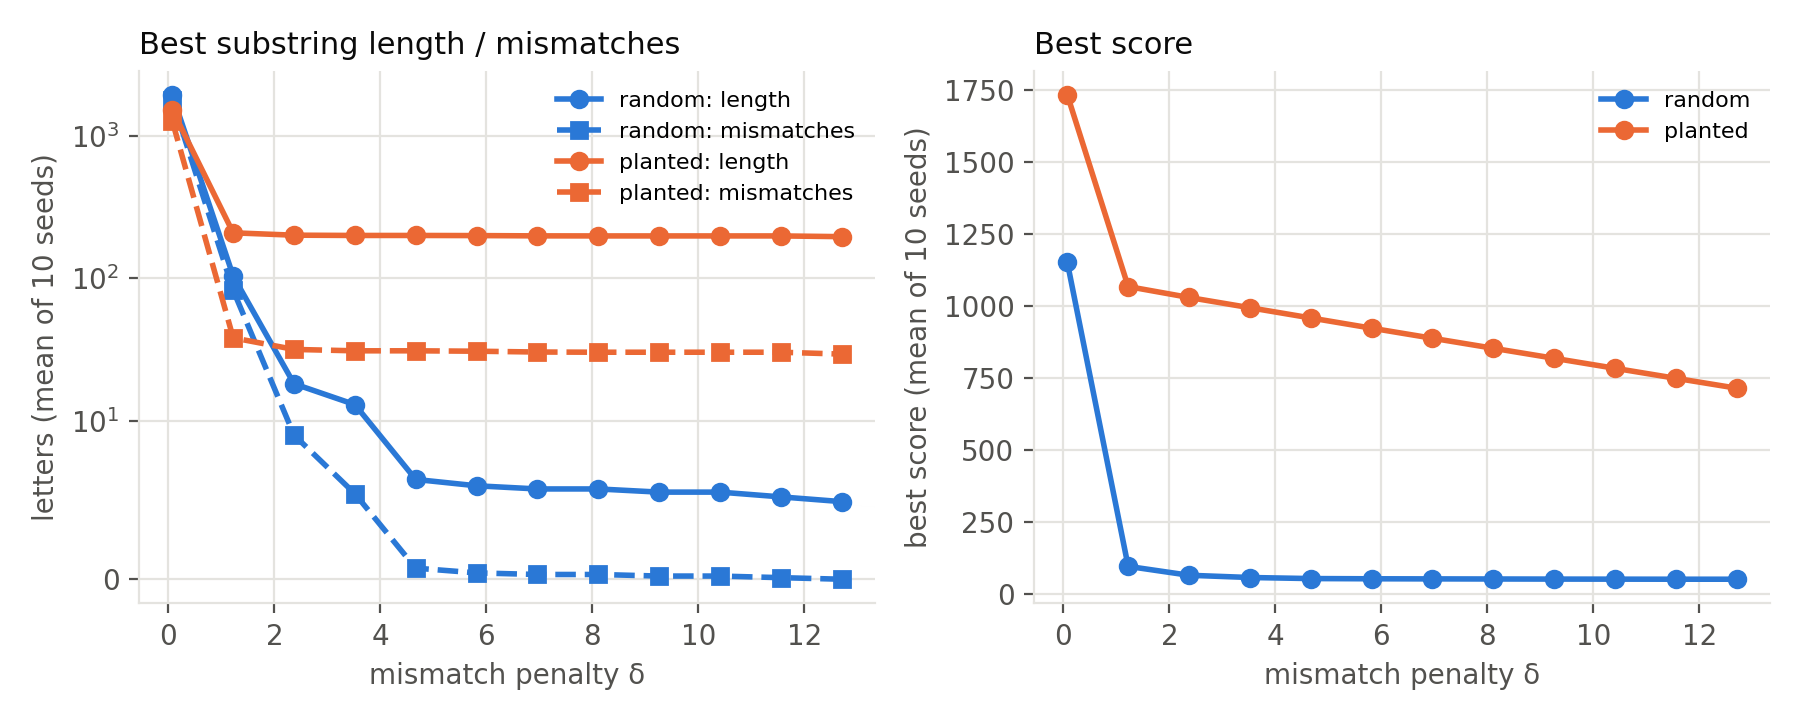
\includegraphics[width=\textwidth]{p1_sweep.png}
\caption{Scenario 2 sweep over $\delta$ (means of 10 seeds). Length and
mismatches on a symlog axis.}\label{fig:p1sweep}
\end{figure}

\paragraph{Observations.}
\begin{itemize}
\item When $\delta$ is close to $w_{\min}$, a mismatch costs less than almost any
  match gains. The optimum then spans most of the overlap of the two strings
  (about 1900 letters, mostly mismatches) and is not meaningful. This is the
  degenerate end of the range.
\item On random strings the optimum shrinks quickly as $\delta$ grows. Once
  $\delta\gtrsim 4.7$ it is a short (5--7 letter) nearly exact match made of
  high-weight letters (E, T, A, O, \dots). At $\delta=w_{\max}$ the
  optimum is an exact match in every seed.
\item On planted data, every $\delta\ge 1.2$ recovers the planted block almost
  exactly (length $\approx200$, about 30 mismatches, overlap $\approx198$--$199$ of 200).
  A mutated region can be found as long as the penalty does not exceed the
  typical gain of the matched letters between two mismatches. The score
  decreases linearly in $\delta$ (slope $\approx -31$, the number of
  mismatches), as expected from the definition.
\item For comparison, Scenario~1 ($w=1,\delta=10$) on the same planted data
  returns only a \SOneLen-letter fragment of the block on average
  (\SOneMis{} mismatches, score \SOneScore). A mismatch costs 10 matches, so the
  optimum only bridges a mismatch when there are more than 10 matches between
  two mutations. Uniform weights with a large penalty behave like a
  \emph{longest exact common substring}. For random uniform strings this has
  length about $\log_{26}(nm)\approx 4$--$5$, which matches the
  scores of 3--5 in the Scenario~1 timing runs.
\end{itemize}

\subsubsection{Scenario 1: effect of the penalty (additional experiment)}\label{sec:s1sweep}
The assignment fixes $\delta=10$ for Scenario~1. To see how much this choice
matters, we also repeat the sweep with $w_c=1$ for $\delta\in\{1,2,3,4,5,6,8,10\}$. The set-up is the
same as for Scenario~2 ($n=m=2000$, 10 seeds, \emph{random} and
\emph{planted} data with a 200-letter block mutated at rate 0.15), except
that letters are drawn uniformly from $\{A..Z\}$.

\begin{table}[h]\centering\small
\caption{Scenario 1 ($w_c=1$), $n=m=2000$, means of 10 seeds, for several penalties $\delta$.}\label{tab:p1sweep1}
\begin{tabular}{rrrrrrrr}\toprule
 & \multicolumn{3}{c}{random strings} & \multicolumn{4}{c}{planted 200-letter block, 15\% mutated}\\
\cmidrule(lr){2-4}\cmidrule(lr){5-8}
$\delta$ & score & length & mism. & score & length & mism. & overlap\\\midrule
\tabinput{../results/p1_sweep_s1_table.tex}
\bottomrule\end{tabular}
\end{table}

\begin{figure}[h]\centering
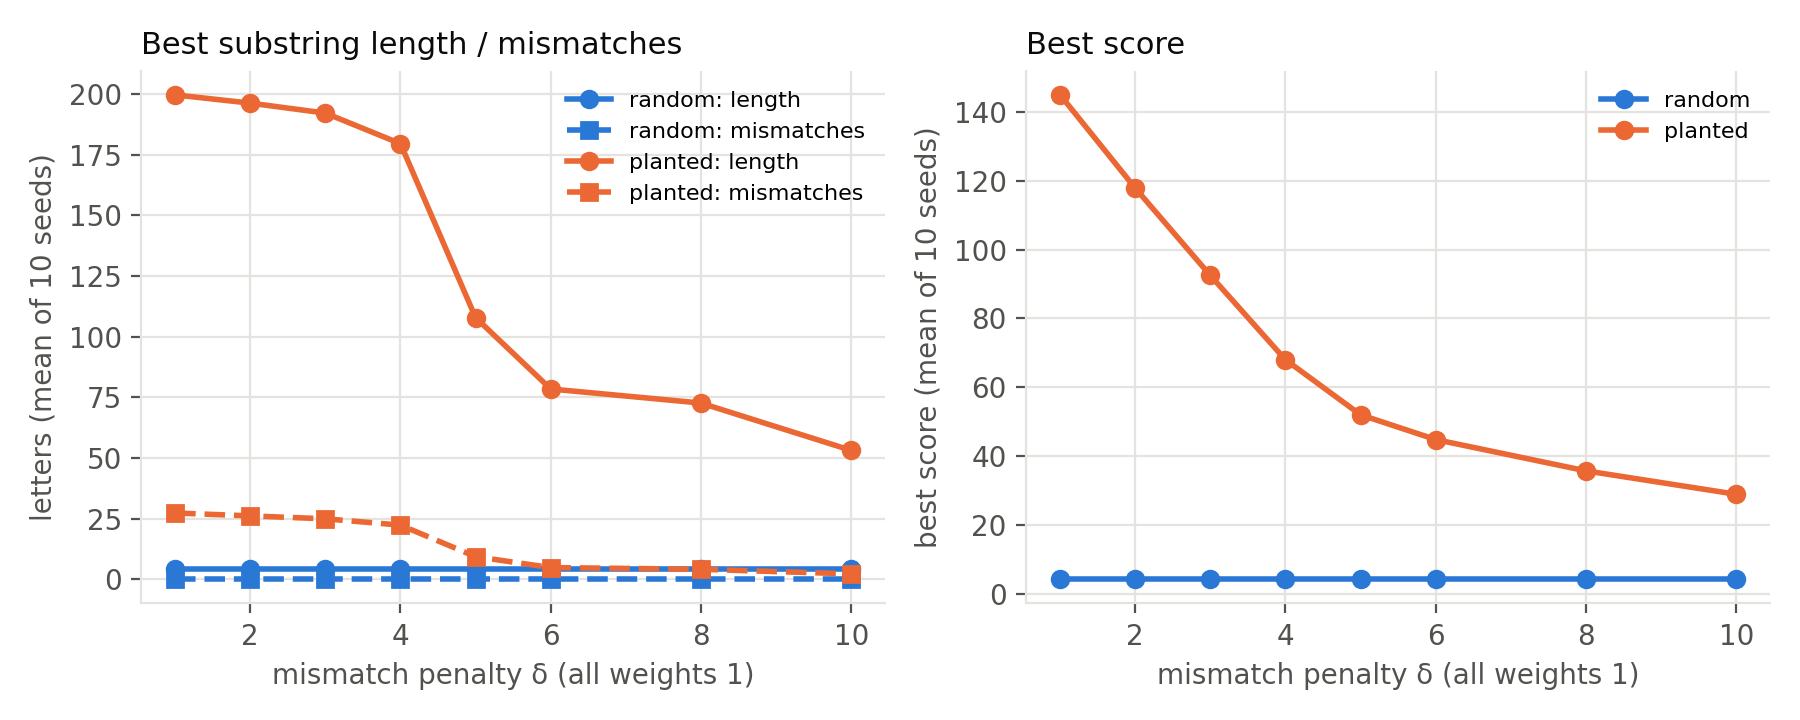
\includegraphics[width=\textwidth]{p1_sweep_s1.png}
\caption{Scenario 1 ($w_c=1$) for several penalties $\delta$ (means of 10 seeds).}\label{fig:p1sweep1}
\end{figure}

\paragraph{Observations.}
\begin{itemize}
\item On random strings the result is the same for every $\delta\ge1$: an
  exact common substring of about 4 letters, with no mismatches. With
  $w_c=1$, joining two exact runs of lengths $a$ and $b$ across one mismatch
  scores $a+b-\delta$, which beats the longer run alone only if the shorter
  run has more than $\delta$ letters. In random text, long runs on the same
  diagonal are very rare, so the optimum is simply the longest exact common
  substring, whatever the penalty.
\item On planted data the penalty decides whether the approximate match is
  found. A fraction $\mu\approx0.14$ of the planted letters are mismatches, so
  along the block the score changes on average by $(1-\mu)\cdot1-\mu\delta$
  per letter. This is positive for
  $\delta<(1-\mu)/\mu\approx 6$. Indeed, for $\delta\le4$ the
  algorithm returns 180--200 letters of the block. Between 5 and 6 the
  answer shrinks, and for $\delta\ge6$ only a fragment between a few mutations
  is reported (53 letters at $\delta=10$).
\item So the conclusions of Scenario~1 depend strongly on the penalty. With
  the assignment's $\delta=10$, Scenario~1 behaves like a longest exact common
  substring and recovers only fragments of a mutated match. For
  a small penalty (around 1--4) the measure tolerates mismatches like
  Scenario~2 does. For a large penalty (6 or more) it behaves like a longest
  exact common substring. The running time does not depend on $\delta$: in this
  sweep the median solve took 5.0--5.4~ms for every penalty.
\end{itemize}

\clearpage
%======================================================================
\section{Problem 2: Largest All-Zero Square Sub-matrix}
%======================================================================

\subsection{Problem statement}
Given an $m\times n$ boolean matrix $B$ (any non-zero value is treated as 1),
find the largest $k$ and a position $(r,c)$ such that $B[r..r+k-1][c..c+k-1]$
is entirely zero ($k=0$ if $B$ has no zero).

\subsection{Optimisation function and Bellman equations}
Let $D[i][j]$ be the side of the largest all-zero square whose
\emph{bottom-right} corner is $(i,j)$ (0-based):
\[
D[i][j] = \begin{cases}
0 & B[i][j]=1,\\
1 & B[i][j]=0 \text{ and } (i=0 \text{ or } j=0),\\
1+\min\bigl(D[i-1][j],\; D[i][j-1],\; D[i-1][j-1]\bigr) & \text{otherwise},
\end{cases}
\]
and the answer is $k^\ast=\max_{i,j} D[i][j]$.

\subsection{Correctness}
\begin{lemma}
For $B[i][j]=0$ and $i,j\ge1$: an all-zero $t\times t$ square ($t\ge2$) has
its bottom-right corner at $(i,j)$ if and only if the three $(t-1)\times(t-1)$
squares with bottom-right corners $(i-1,j)$, $(i,j-1)$ and $(i-1,j-1)$ are all zero.
\end{lemma}
\begin{proof}
($\Rightarrow$) Each of the three smaller squares lies inside the $t\times t$
square. ($\Leftarrow$) The $t\times t$ square with bottom-right corner $(i,j)$
covers rows $i-t+1..i$ and columns $j-t+1..j$. Every cell except $(i,j)$ lies
in at least one of the three smaller squares: the cells of row $i$ (except the
corner) lie in the one ending at $(i,j-1)$, the cells of column $j$ (except the
corner) in the one ending at $(i-1,j)$, and the rest in all three. The
corner itself is zero by assumption.
\end{proof}
\begin{theorem}
$D[i][j]$ as computed equals the true value, and $k^\ast$ is optimal.
\end{theorem}
\begin{proof}
By induction in row-major order. The cases $B[i][j]=1$ and the first row or
column are immediate. Otherwise, a zero square of side $t\ge2$ ends at $(i,j)$
iff (by the lemma) $t-1\le D[i-1][j]$, $t-1\le D[i][j-1]$ and
$t-1\le D[i-1][j-1]$. The largest such $t$ is $1+\min(\cdot)$. Every square
has a bottom-right corner, so $k^\ast=\max D$ is optimal.
\end{proof}

\subsection{Extracting the optimal square}
While filling the table we record the first cell $(i^\ast,j^\ast)$ in row-major
order that attains the maximum. The optimal square is
\[
\text{rows } i^\ast-k^\ast+1 \,..\, i^\ast,\qquad \text{columns } j^\ast-k^\ast+1 \,..\, j^\ast .
\]
Extraction needs only $(k^\ast,i^\ast,j^\ast)$, so it works the same with the full table or
with two rolling rows. The tests check that every reported square is
inside the matrix and all zero.

\subsection{Storage: one byte per value}
$B$ is stored as one Java \texttt{byte} per cell. A DP value never
exceeds $\min(m,n)$. Following the hint, the table is a \texttt{byte[]}
whenever $\min(m,n)\le255$. Java's \texttt{byte} is signed ($-128..127$), so
values are read back as unsigned with \texttt{d \& 0xFF}, which gives the full
range $0..255$. This covers the $10\times10$, $10\times100$,
$10\times1000$ and $100\times1000$ cases. A single byte \emph{cannot} hold the
answer in general when $\min(m,n)>255$: an all-zero $1000\times1000$ matrix has
$k^\ast=1000$. So the program selects the cell type at run time:
a \texttt{short[]} read as unsigned (\texttt{\& 0xFFFF}) for
$\min(m,n)\le65535$, and an \texttt{int[]} beyond that. The test suite
includes an all-zero $200\times200$ matrix ($k^\ast=200>127$, which checks the
unsigned reading) and an all-zero $300\times400$ matrix ($k^\ast=300$, which
would silently overflow with bytes).

\subsection{Time and space complexity}
\begin{itemize}
\item \textbf{Time} $\Theta(mn)$: each of the $mn$ cells needs one test and a
  minimum of three neighbours. Extraction is $O(1)$.
\item \textbf{Space}: the input takes $mn$ bytes. The full DP table takes
  $mn\cdot\lceil\log_{256}(\min(m,n)+1)\rceil$ bytes, so $mn$ bytes for the
  four smaller required sizes. The rolling-row variant needs only
  $2n$ \texttt{int}s ($8n$ bytes), $\Theta(n)$ (or $\Theta(\min(m,n))$ by transposing). In total
  this is $\Theta(mn)$ because of the input. Packing the input as bits would
  reduce the input to $mn/8$ bytes without changing the asymptotics.
\end{itemize}

\subsection{Experiments}
\paragraph{Data.} For each of the five required sizes, $10\times10$,
$10\times100$, $10\times1000$, $100\times1000$ and $1000\times1000$, every cell
is set to 1 independently with probability $p$. We use three densities,
$p\in\{0.5, 0.1, 0.01\}$, because with $p=0.5$ the largest zero square is tiny
($k\le4$). Smaller $p$ gives larger squares. Timing repeats each solve until at
least 50~ms have elapsed and takes the mean per solve, and reports the best of
5 such trials. This gives stable values for sub-microsecond inputs. Memory is
reported in two ways ($p=0.1$). (i) The computed size of the arrays (cells
$\times$ bytes per cell). (ii) The heap bytes \emph{measured} by the JVM
(\texttt{ThreadMXBean.getCurrentThreadAllocatedBytes}) while generating $B$
and while solving. The measured numbers include Java object headers and the
small result object. Measuring the whole JVM process (tens of MiB for the
runtime itself) would hide arrays of a few hundred bytes completely.

\paragraph{Correctness tests.} \texttt{java ZeroSquare test} checks a hand
example, an all-ones matrix, single rows and columns, the byte-overflow case
and 3000 random matrices up to $15\times15$. It compares the full DP, the
rolling DP and a brute force that tries every corner and size. All tests pass.

\begin{table}[h]\centering\small
\caption{Problem 2 running time ($\mu$s) of the full-table DP, and the side $k^\ast$ found, for three densities. The last column is the two-row variant at $p=0.1$.}
\begin{tabular}{lrrrrrrr}\toprule
 & \multicolumn{2}{c}{$p=0.5$} & \multicolumn{2}{c}{$p=0.1$} & \multicolumn{2}{c}{$p=0.01$} & rolling\\
\cmidrule(lr){2-3}\cmidrule(lr){4-5}\cmidrule(lr){6-7}\cmidrule(lr){8-8}
$m\times n$ & $\mu$s & $k^\ast$ & $\mu$s & $k^\ast$ & $\mu$s & $k^\ast$ & $\mu$s\\\midrule
\tabinput{../results/p2_runtime_table.tex}
\bottomrule\end{tabular}
\end{table}

\begin{table}[h]\centering\small
\caption{Problem 2 memory in bytes ($p=0.1$): computed array sizes, and heap allocation measured by the JVM.}
\begin{tabular}{lrrrrrr}\toprule
 & \multicolumn{3}{c}{computed (bytes)} & \multicolumn{3}{c}{measured heap allocation (bytes)}\\
\cmidrule(lr){2-4}\cmidrule(lr){5-7}
$m\times n$ & input $B$ & full DP & 2-row DP & input $B$ & solve, full & solve, 2-row\\\midrule
\tabinput{../results/p2_memory_table.tex}
\bottomrule\end{tabular}
\end{table}

\begin{figure}[h]\centering
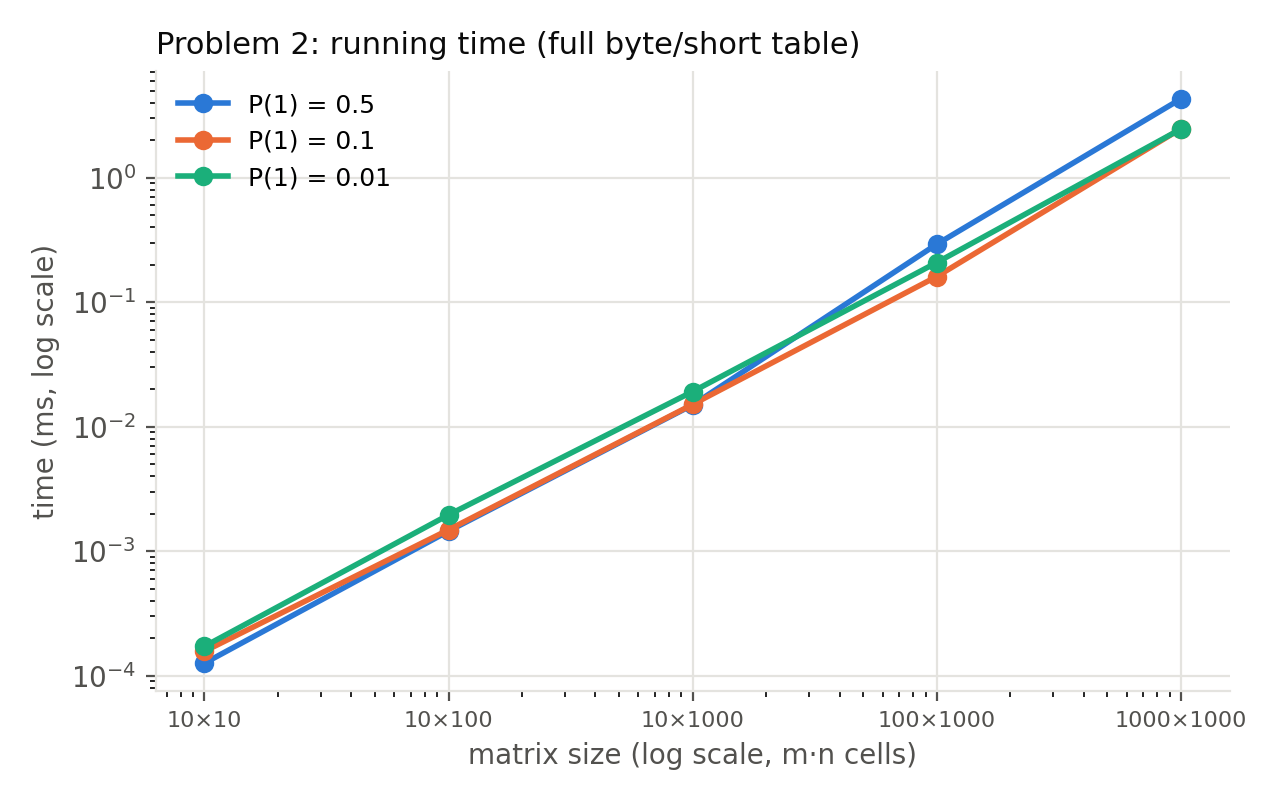
\includegraphics[width=0.7\textwidth]{p2_runtime.png}
\caption{Problem 2 running time (log--log). Slope 1 means time is linear in the number of cells $mn$.}\label{fig:p2rt}
\end{figure}

\begin{figure}[h]\centering
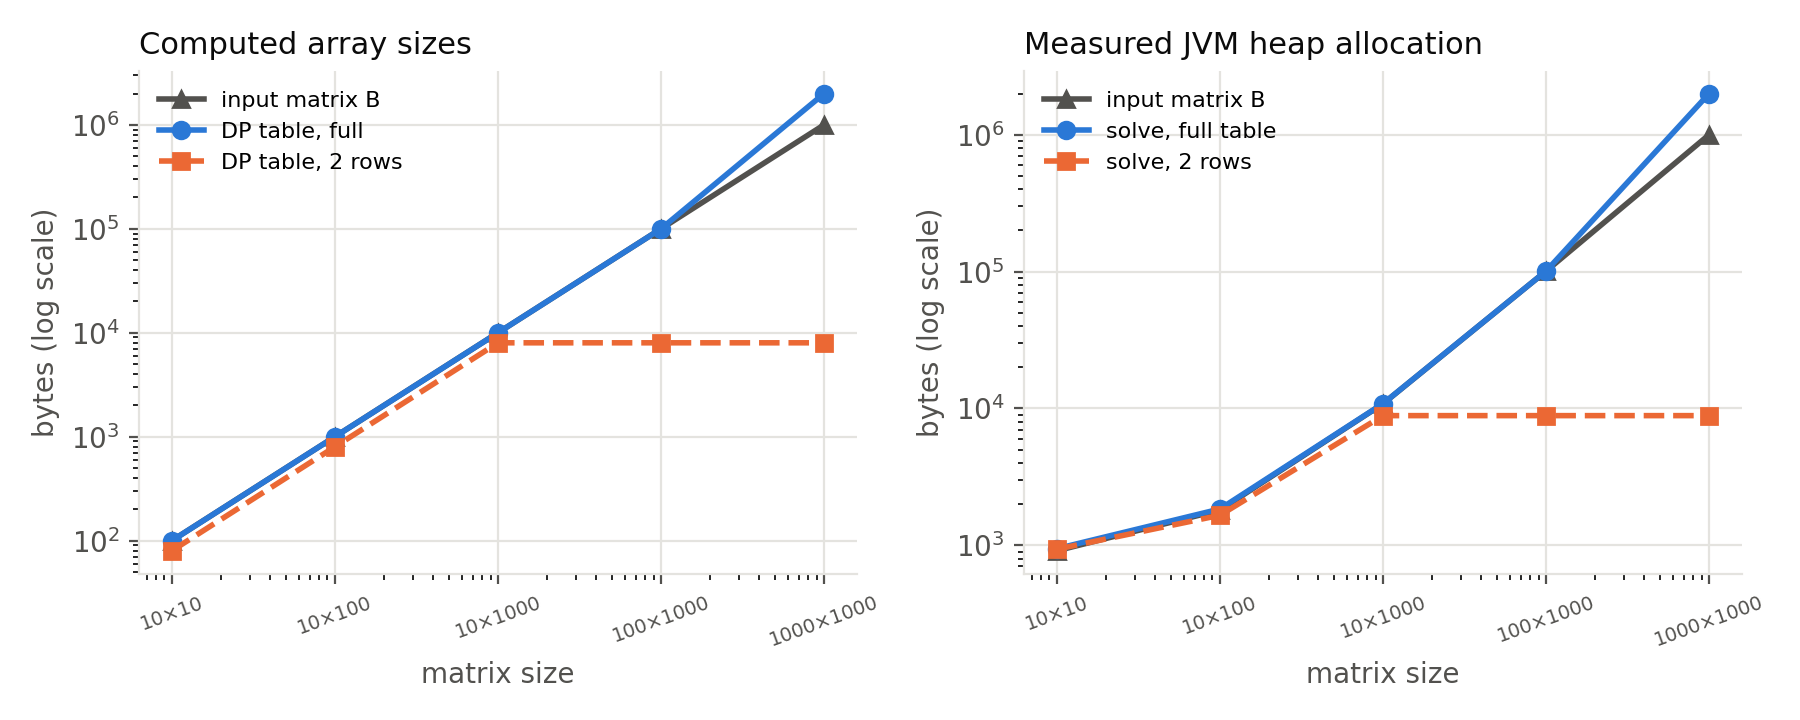
\includegraphics[width=\textwidth]{p2_memory.png}
\caption{Problem 2 memory (log scale). Left: computed array sizes. Right: heap bytes measured by the JVM.}\label{fig:p2mem}
\end{figure}

\paragraph{Observations.}
\begin{itemize}
\item Each 10$\times$ increase in the number of cells increases the time
  about 10$\times$ (slope 1 on the log--log plot), as predicted by $\Theta(mn)$.
  Solving $10^6$ cells takes about 2.5--4.3~ms. The time per cell grows
  slightly from the small to the large matrices (1.5 to 2.5~ns at $p=0.1$).
  This is a constant-factor effect of the memory hierarchy, not a change in
  growth rate.
\item At $p=0.5$ the two larger sizes are about 1.7--1.8$\times$ slower than at
  $p=0.1$ or $0.01$, even though the operation count is identical. With
  $p=0.5$ the branch ``$B[i][j]=1$?'' is a coin flip, so the CPU's branch
  predictor fails about half the time. The effect is a constant factor and does
  not change the asymptotic growth. In our runs it appears only for the two
  largest sizes, and we did not investigate where it starts.
\item Allocated memory follows the analysis exactly. The full table equals
  $mn$ bytes for the four smaller sizes and $2mn$ bytes (\texttt{short})
  for $1000\times1000$. The two-row table takes $8n$ bytes.
\item The measured heap allocation equals the computed size plus a constant
  of under 1~KB: a 16-byte array header per array, the result object, and
  JVM bookkeeping. At $1000\times1000$ the full table allocates 2{,}000{,}840
  bytes against 2{,}000{,}000 computed, and the two-row version 8{,}856 bytes
  against 8{,}000. The memory used by the full method grows linearly with
  $mn$, while the two-row method grows only with $n$.
\item The two-row variant was about 2$\times$ slower than the full table in
  Java. It stores \texttt{int}s and swaps two array references every row,
  which the JIT appears to optimise less well. We did not investigate this
  further. The asymptotic behaviour is the same.
\end{itemize}


\begin{thebibliography}{9}
\bibitem{lewand} R.~E. Lewand, \emph{Cryptological Mathematics}, Mathematical Association of America, 2000 (letter frequencies as tabulated in ``Letter frequency'', Wikipedia, accessed Oct.\ 2026).
\bibitem{clrs} T.~H. Cormen, C.~E. Leiserson, R.~L. Rivest and C.~Stein, \emph{Introduction to Algorithms}, 3rd ed., MIT Press, 2009.
\bibitem{kt} J.~Kleinberg and \'E.~Tardos, \emph{Algorithm Design}, Pearson, 2006.
\end{thebibliography}

\appendix
\section{Source Code}
\subsection{Problem 1: \texttt{src/Substring.java}}
\lstinputlisting{../src/Substring.java}
\subsection{Problem 2: \texttt{src/ZeroSquare.java}}
\lstinputlisting{../src/ZeroSquare.java}

\end{document}
